\documentclass[twoside, a4paper, titlepage]{article}
\usepackage[utf8]{inputenc}
\usepackage[T1]{fontenc}
\usepackage{amsmath}
\usepackage{mathtools}
\usepackage[french]{cleveref}
\usepackage[french]{babel}
\usepackage[listings,theorems,most]{tcolorbox}

\newtcolorbox[use counter=equation]{equationEncadree}[1][]{colback=blue!5!white,
   colframe=blue!75!black,
   fonttitle=\bfseries, 
   title=Équation importante~\theequation~,
   #1}

\counterwithin{equation}{section} %on ajoute le numéro de section devant le numéro d'équation

\newtcolorbox[blend into=figures]{customFig}[2][]{float=hbtp,
    blend before title=colon hang,
    colframe=yellow!75!black,
    colback=yellow!5!white,
    fonttitle=\bfseries,
    title= {#2},
    every float=\centering,
    halign=flush center,
    halign lower=flush center,
    lower separated=false,
    #1}

\counterwithin{figure}{section}

\newtcolorbox[auto counter,
   number within=section,
   crefname={résultat}{résultats},
   Crefname={Résultat}{Résultats}]
   {resultat}[2][]
   {colback=red!5!white, 
   colframe=red!75!black,
   fonttitle=\bfseries, 
   title=Résultat~\thetcbcounter~:~{#2},
   #1}

\newtcolorbox[auto counter,
      number within=section,
      crefname={théroème}{théroèmes},
      Crefname={Théroème}{Théroèmes}]
   {theoremCustom}[2][]
   {colback=green!5!white, 
      colframe=green!75!black,
      fonttitle=\bfseries, 
      title=Théorème~\thetcbcounter~:~{#2},
      #1}

\title{Boîte à outils pour des rapports LaTeX}
\author{Ternoc}
\date{9 octobre 2022}

\begin{document}
\maketitle
\tableofcontents
\newpage
   \section{Plusieurs exemples}      
      \subsection{Équation encadrée}
         \begin{equation} \label{eqPasEncadre}
            A=\sqrt{B^2+C^2}
         \end{equation}

         \begin{equationEncadree}[label=eqPremierEncadre]
            \[
               f(x) = x^2
            \]
         \end{equationEncadree}
      
      \subsection{Image}
      Voici l'image de la caméra :
      %\begin{customFig}[sidebyside]{Photo de la caméra}
      \begin{customFig}[label=imgTest]{Photo de la caméra}
         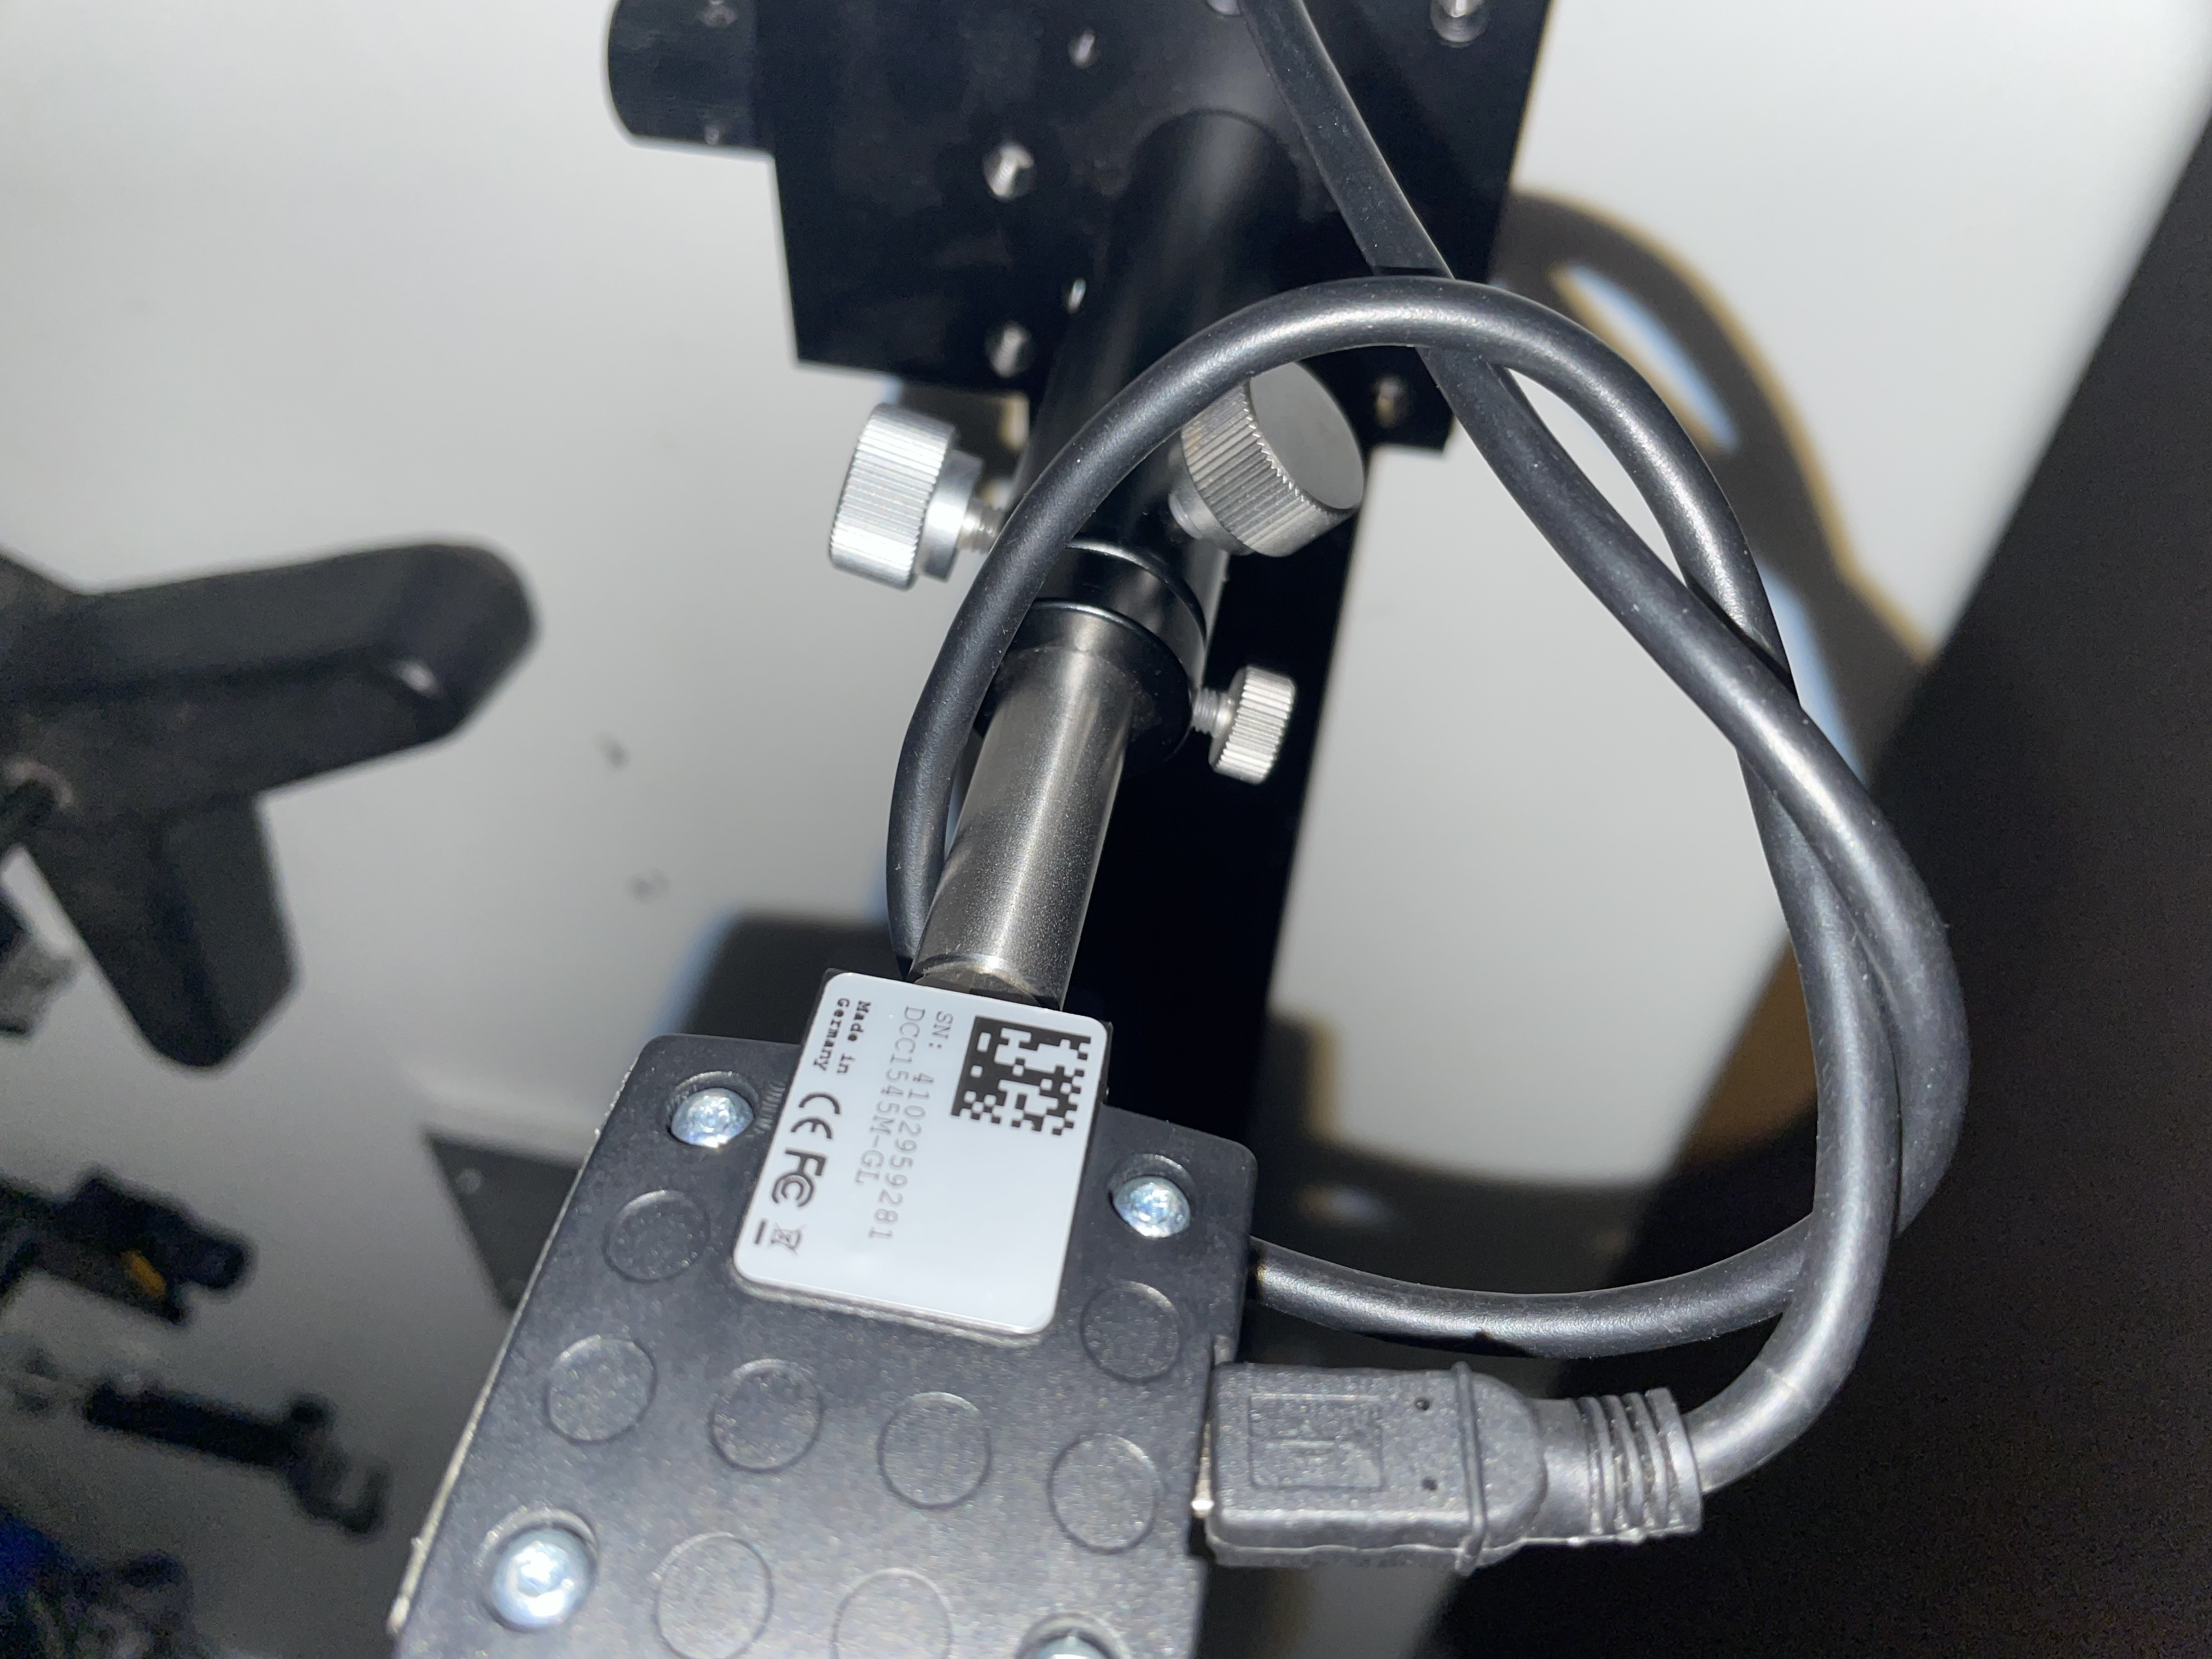
\includegraphics[height=5cm]{IMG_test.jpeg}
         \tcblower
         La photo de la caméra n'est pas très bien.
      \end{customFig}

      \subsection{Encadré personnalisé}
      \begin{resultat}[label=resultat]{Base de travail}
         \[
            \frac{A}{B}=\Delta X
         \]
      \end{resultat}

      \begin{theoremCustom}[label=th]{Théorème de machin}
         \[
            A=\sqrt{\epsilon_0 \mu_0}
         \]
         \tcblower
         On apprend ainsi à quoi correspond $A$
      \end{theoremCustom}
   
   \section{Citations}
   Nous pouvons citer plusieurs choses : \cref{eqPasEncadre}, \cref{eqPremierEncadre}, \cref{imgTest}.

   Mais aussi : \cref{resultat} et \cref{th}
\end{document}